\documentclass[12pt, a4paper]{extarticle}
\usepackage{GOST}
\usepackage{array}
\usepackage{verbatim}
\usepackage[detect-all]{siunitx}
\usepackage{amsmath}
\usepackage{amssymb}
\usepackage[utf8]{inputenc}
\usepackage{hyperref}
\usepackage{tempora}

\makeatletter
\renewcommand\@biblabel[1]{#1.}
\makeatother

\usepackage{listings}
\lstset{ 
	language=Prolog,
	basicstyle=\small, 
	numbers=left, 
	numberstyle=\tiny,
	stepnumber=1,
	numbersep=5pt,
	showspaces=false,            
	showstringspaces=false,      
	showtabs=false,             
	frame=single,            % рисовать рамку вокруг кода
	tabsize=4,      
	commentstyle=\color{green},
	keywordstyle=\color{blue}\textbf,
	numberstyle=\scriptsize\color{gray}, % the style that is used for the line-numbers
	rulecolor=\color{black},
	captionpos=t,
	breaklines=true,         % автоматически переносить строки 
	breakatwhitespace=false, % переносить строки по пробелу
	%escapeinside={\#*}{*)} 
}




\begin{document}
	
\begin{table}[ht]
	\centering
	\begin{tabular}{|c|p{400pt}|} 
		\hline
		\begin{tabular}[c]{@{}c@{}} 
\includegraphics[scale=1]{source/b_logo.jpg} \\\end{tabular} &
		\footnotesize\begin{tabular}[c]{@{}c@{}}\textbf{Министерство~науки~и~высшего~образования~Российской~Федерации}\\\textbf{Федеральное~государственное~бюджетное~образовательное~учреждение}\\\textbf{~высшего~образования}\\\textbf{«Московский~государственный~технический~университет}\\\textbf{имени~Н.Э.~Баумана}\\\textbf{(национальный~исследовательский~университет)»}\\\textbf{(МГТУ~им.~Н.Э.~Баумана)}\\\end{tabular}  \\
		\hline
	\end{tabular}
\end{table}
\noindent\rule{\textwidth}{4pt}
\noindent\rule[14pt]{\textwidth}{1pt}
\hfill 
\noindent
\makebox{ФАКУЛЬТЕТ~}%
\makebox[\textwidth][l]{\underline{~«Информатика и системы управления»~~~~~~~~~~~~~~~~~~~~~~~~~~~~~~~~~}}%
\\
\noindent
\makebox{КАФЕДРА~}%
\makebox[\textwidth][l]{\underline{~«Программное обеспечение ЭВМ и информационные технологии»~}}%
\\

\begin{center}
	\vspace{1.5cm}
	{\bf\huge Отчёт\par}
	{\bf\Large по лабораторной работе № 16\par}
	\vspace{0.7cm}
\end{center}


\noindent
\makebox{\large{\bf Название:}~~~}
\makebox[\textwidth][l]{\large\underline{~Использование правил в программе на Prolog~}}\\

\noindent
\makebox{\large{\bf Дисциплина:}~~~}
\makebox[\textwidth][l]{\large\underline{~Функциональное и логическое программирование~}}\\

\vspace{1.5cm}
\noindent
\begin{tabular}{l c c c c c}
	Студент      & ~ИУ7-65Б~               & \hspace{2.5cm} & \hspace{2cm}                 & &  Д.В. Сусликов \\\cline{2-2}\cline{4-4} \cline{6-6} 
	\hspace{3cm} & {\footnotesize(Группа)} &                & {\footnotesize(Подпись, дата)} & & {\footnotesize(И.О. Фамилия)}
\end{tabular}

\noindent
\begin{tabular}{l c c c c}
	Преподаватель & \hspace{5cm}   & \hspace{2cm}                 & & ~~~~~~Н.Б. Толпинская~~~~~~\\\cline{3-3} \cline{5-5} 
	\hspace{3cm}  &                & {\footnotesize(Подпись, дата)} & & {\footnotesize(И.О. Фамилия)}
\end{tabular}

\vspace{0.6cm}
\begin{center}	
	\vfill
	\large \textit {Москва, 2021}
\end{center}

\thispagestyle {empty}
\pagebreak

\clearpage

\textbf{Задание}\par

Создать базу знаний: <<ПРЕДКИ>>, позволяющую наиболее эффективным способом (за меньшее количество шагов, что обеспечивается меньшим количеством предложений БЗ - правил), используя разные варианты (примеры) одного вопроса, определить (указать: какой вопрос для какого варианта):
\begin{enumerate}
	\item по имени субъекта определить всех его бабушек (предки 2-го колена),
	\item по имени субъекта определить всех его дедушек (предки 2-го колена),
	\item по имени субъекта определить всех его бабушек и дедушек (предки 2-го колена),
	\item по имени субъекта определить его бабушку по материнской линии (предки 2-го колена),
	\item по имени субъекта определить его бабушку и дедушку по материнской линии (предки 2-го колена).
\end{enumerate}

Минимизировать количество правил и количество вариантов вопросов. Использовать конъюнктивные правила и простой вопрос.

Для одного из вариантов вопроса и конкретной БЗ составить таблицу, отражающую конкретный порядок работы системы

\hfill

\textbf{Листинг:}

\begin{lstlisting}
domains
	name = symbol.
predicates
	dad(name, name).
	mom(name, name).
	all_granddad(name, name).
	all_grandma(name, name).
	all_grandparents(name, name).
	grandma_M(name, name).
	granddad_M(name, name).
	grandma_F(name, name).
	granddad_F(name, name).
	grandparents_M(name, name).

clauses
	dad("Vlad", "Danya").
	dad("Vova", "Vlad").
	dad("Yuri", "Diana").
	dad("Yuri", "Dima").
	mom("Diana", "Danya").	
	mom("Tonya", "Vlad").
	mom("Lyuda", "Diana").
	
	grandma_M(Grandma, Sub):- mom(Mom, Sub), !, mom(Grandma, Mom), !.
	granddad_M(Granddad, Sub):- mom(Mom, Sub), !, dad(Granddad, Mom), !.
	
	grandma_F(Grandma, Sub):- dad(Dad, Sub), !, mom(Grandma, Dad), !.
	granddad_F(Granddad, Sub):- dad(Dad, Sub), !, dad(Granddad, Dad), !.
	
	all_grandma(Grandma, Sub):- grandma_M(Grandma, Sub).
	all_grandma(Grandma, Sub):- grandma_F(Grandma, Sub).
	
	all_granddad(Granddad, Sub):- granddad_M(Granddad, Sub).
	all_granddad(Granddad, Sub):- granddad_F(Granddad, Sub).
	
	all_grandparents(Grandparent, Sub):- all_grandma(Grandparent, Sub).
	all_grandparents(Grandparent, Sub):- all_granddad(Grandparent, Sub).
	
	grandparents_M(Grand, Sub):- grandma_M(Grand, Sub).
	grandparents_M(Grand, Sub):- granddad_M(Grand, Sub).

goal
	%all_grandma(Grandma, "Danya").
	%all_granddad(GrandPa, "Danya").
	%all_grandparents(Grand, "Danya").
	%grandma_M(Grandma, "Danya").
	%grandparents_M(Grand, "Danya").
\end{lstlisting}
\newpage

Результаты работы:\par
\begin{figure}[h!]
	\begin{minipage}[h]{0.48\linewidth}
		\center{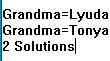
\includegraphics[width=0.48\linewidth]{source/1.png} \\ Пример all\_grandma}	
	\end{minipage}
	\hfill
	\begin{minipage}[h]{0.48\linewidth}
		\center{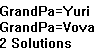
\includegraphics[width=0.48\linewidth]{source/2.png} \\ Пример all\_granddad}	
	\end{minipage}
\end{figure}\par

\begin{figure}[h!]
	\begin{minipage}[h]{0.48\linewidth}
		\center{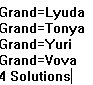
\includegraphics[width=0.48\linewidth]{source/3.png} \\ Пример all\_grandparents}	
	\end{minipage}
	\hfill
	\begin{minipage}[h]{0.48\linewidth}
		\center{
\includegraphics[width=0.48\linewidth]{source/4.png} \\ Пример grandma\_M}	
	\end{minipage}
\end{figure}\par

\begin{figure}[h!]	
	\center{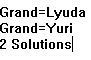
\includegraphics{source/5.png} \\ Пример grandparents\_M}	
\end{figure}\par

\newpage
\textbf{Приведем таблицу для поиска бабушки по линии матери. }\par
grandma\_M(Grandma, "Danya")\par

\begin{table}[h!]
	\begin{tabular}{|l|l|l|l|}
		\hline
		\begin{tabular}[c]{@{}l@{}}№\\ шага\end{tabular} & \begin{tabular}[c]{@{}l@{}}Состояние резольвенты\\ и вывод\end{tabular}               & \begin{tabular}[c]{@{}l@{}}Для каких термов запускается\\ алгоритм унификации и каков\\ результат\end{tabular}                                                                            & Дальнейшие действия                                                                \\ \hline
		0                                                & \begin{tabular}[c]{@{}l@{}}grandma\_M(Grandma,\\ "Danya")\end{tabular}                &                                                                                                                                                                                           &                                                                                    \\ \hline
		1                                                & \begin{tabular}[c]{@{}l@{}}grandma\_M(Grandma,\\ "Danya")\end{tabular}                & \begin{tabular}[c]{@{}l@{}}T1 = grandma\_M(Grandma, "Danya")\\ T2 = dad(...)\\ Неудача. Не унифицируемы.\end{tabular}                                                                     & \begin{tabular}[c]{@{}l@{}}Переход к следующему\\ заголовку БЗ\end{tabular}        \\ \hline
		& ...                                                                                   & ...                                                                                                                                                                                       & ...                                                                                \\ \hline
		2                                                & \begin{tabular}[c]{@{}l@{}}grandma\_M(Grandma,\\ "Danya")\end{tabular}                & \begin{tabular}[c]{@{}l@{}}Т1 = grandma\_M(Grandma, "Danya")\\ Т2 = grandma\_M(Grandma, Sub)\\ Успех. Унифицируемы.\\ \\ Подстановка:\\ \{Grandma = Grandma, Sub = "Danya"\}\end{tabular} & \begin{tabular}[c]{@{}l@{}}Замена на тело\\ предложения\end{tabular}               \\ \hline
		3                                                & \begin{tabular}[c]{@{}l@{}}mom(Mom, "Danya"), !, \\ mom(Grandma, Mom), !\end{tabular} & \begin{tabular}[c]{@{}l@{}}T1 = mom(Mom, "Danya")\\ T2 = dad(...)\\ Неудача. Не унифицируемы.\end{tabular}                                                                                & \begin{tabular}[c]{@{}l@{}}Переход к следующему\\ заголовку БЗ\end{tabular}        \\ \hline
		& ...                                                                                   & ...                                                                                                                                                                                       & ...                                                                                \\ \hline
		4 & \begin{tabular}[c]{@{}l@{}}mom(Mom, "Danya"), !, \\ mom(Grandma, Mom), !\end{tabular} & \begin{tabular}[c]{@{}l@{}}T1 = mom(Mom, "Danya")\\ T2 = mom("Diana", "Danya")\\ Успех Унифицируемы.\\ \\ Подстановка:\\ \{Mom = "Diana", "Danya" = "Danya"\}\end{tabular}                & \begin{tabular}[c]{@{}l@{}}Замена на тело\\ предложения\\ (на пустое)\end{tabular} \\ \hline
		5 & \begin{tabular}[c]{@{}l@{}}!, \\ mom(Grandma, Mom), !\end{tabular}                    & \begin{tabular}[c]{@{}l@{}}!\\ Истина\end{tabular}                                                                                                                                        & \begin{tabular}[c]{@{}l@{}}Замена на тело\\ предложения\\ (на пустое)\end{tabular} \\ \hline
	\end{tabular}
\end{table}

\newpage

\begin{table}[h!]
	\begin{tabular}{|l|l|l|l|}
		\hline
		6  & mom(Grandma, "Diana"), ! & \begin{tabular}[c]{@{}l@{}}T1 = mom(Grandma, "Diana")\\ T2 = dad(...)\\ Неудача. Не унифицируемы.\end{tabular}                                                                     & \begin{tabular}[c]{@{}l@{}}Переход к следующему\\ заголовку БЗ\end{tabular}        \\ \hline
		& ...                      & ...                                                                                                                                                                                & ...                                                                                \\ \hline
		7  & mom(Grandma, "Diana"), ! & \begin{tabular}[c]{@{}l@{}}T1 = mom(Grandma, "Diana")\\ T2 = mom("Lyuda", "Diana")\\ Успех. Унифицируемы.\\ \\ Подстановка:\\ \{Grandma = "Lyuda", "Diana" = "Diana\}\end{tabular} & \begin{tabular}[c]{@{}l@{}}Замена на тело\\ предложения\\ (на пустое)\end{tabular} \\ \hline
		8  & !                        & \begin{tabular}[c]{@{}l@{}}!\\ Истина\end{tabular}                                                                                                                                 & \begin{tabular}[c]{@{}l@{}}Замена на тело\\ предложения\\ (на пустое)\end{tabular} \\ \hline
		9  & \begin{tabular}[c]{@{}l@{}}Резольвента пуста.\\ Вывод\\ Grandma = "Lyuda"\end{tabular}      &                                                                                                                                                                                    & \begin{tabular}[c]{@{}l@{}} Откат\end{tabular}       \\ \hline
		10 & !                        & \begin{tabular}[c]{@{}l@{}}!\\ Завершение процедуры\end{tabular}                                                                                                                   & \begin{tabular}[c]{@{}l@{}}Замена на тело\\ предложения\\ (на пустое)\end{tabular} \\ \hline
		11 & Резольвента пуста        &                                                                                                                                                                                    & \begin{tabular}[c]{@{}l@{}}Завершение работы\\ программы\end{tabular}              \\ \hline
	\end{tabular}
\end{table}
\newpage

\textbf{Ответы на вопросы}\par

\begin{enumerate} 
	
	\item[1)] В каком случае система запускает алгоритм унификации? (Как эту необходимость на формальном уровне распознает система?)
	
	Системы запускате алгоритм унификации, пока резольвента не пуста.
	
	\item[2)] Каковы назначение и результат использования алгоритма унификации? 
	
	Алгоритм унификации необходим для того, чтобы подобрать знание, чтобы
	ответить на поставленный вопрос. Результатом работы алгоритма является
	значение переменной «неудача». Если неудача = 1, то унификация невозможна;
	если неудача = 0, то унификация прошла успешно, а побочным действием работы
	алгоритма является содержимое результирующей ячейки – результирующая
	подстановка.
	
	\item[3)] Какое первое состояние резольвенты?
	
	Вопрос. 
	
	\item[4)] Как меняется резольвента?
	
	Резольвента меняется в 2 этапа:
	\begin{itemize}
		\item Редукция (замена вопроса на тело правила, заголовок которого был успешно унифицирован);
		\item Применение подстановки.
	\end{itemize}
	
	\item[5)] В каких пределах программы уникальны переменные? 
	
	Именованные переменные уникальны в рамках предложения, анонимные --  везде.
		
	\item[6)] Как применяется подстановка, полученная с помощью алгоритма унификации?
	
	В результате подстановки связываются переменные, которые еще не были
	связаны. После связывания всех утверждений, будет напечатано значение
	связанных переменных.
	
	\item[7)] В каких случаях запускается механизм отката?
	
	В случае, когда унификация на текущем шаге завершается тупиковой
	ситуацией, или был получен ответ «да».	
\end{enumerate}

\end{document}